\chapter{Конструкторский раздел}%
\label{cha:konstruktorskii_razdel}

В данном разделе рассматривается структура программного обеспечения.

\section{Состав программного обеспечения}%
\label{sec:sostav_programmnogo_obespecheniia}

Программное обеспечение состоит из загружаемого модуля ядра.

Для компиляции модуля используется Makefile. В листинге~\ref{lst:makefile} представлен makefile, с помощью которого компилировался модуль ядра из данной работы.
\begin{lstlisting}[language=make,caption={Makefile},label=lst:makefile]
CONFIG_MODULE_SIG=n
ldflags-y += -T$(src)/3rd_party/khook/engine.lds

ifneq ($(KERNELRELEASE),)
	obj-m := fnrootkit.o
	fnrootkit-objs := ./src/net.o ./src/proc.o ./src/fnrootkit.o
else
	CFLAGS += -Wall
	CC := gcc $(CFLAGS)
	PWD := $(shell pwd)
	KDIR := /lib/modules/$(shell uname -r)/build

all:
	$(MAKE) -C $(KDIR) M=$(PWD) modules

clean:
	$(MAKE) -C $(KDIR) M=$(PWD) clean
endif
\end{lstlisting}

\section{Скрытие загружаемого модуля ядра}%
\label{sec:skrytie_zagruzhaemogo_modulia_iadra}

Загруженные модули ядра можно просмотреть с помощью команды lsmod. lsmod это простая утилита, которая не принимает никаких опций или аргументов. Команда выполняет то, что читает /proc/modules и отображает содержимое файла в хорошо отформатированном списке.

Для реализации скрытого руткита необходимо удалить загружаемый модуль с рутиктом из основного списка модулей.

В Linux модуль ядра описывается структурой struct module. Как и многие другие сущности ядра, модули хранятся в списках беркли. Для взаимодействия со списками беркли необходимо использовать структуру list\_head. Удаление из списка происходит с помощью функции list\_del.

Перед удалением загружаемого модуля ядра из списка необходимо сохранить его указатель на этот модуль, чтобы в дальнейшем, во время выгрузки модуля ядра, можно было вернуть модуль в список.

\section{Скрытие процессов}%
\label{sec:skrytie_protsessov}

В результате анализа системных вызовов, которые использует утилита ps, с помощью утилиты strace, описание которой представлено в аналитическом разделе, было выявлено, что каждая операция по перечислению процессов требует использование системного вызова getdents64 (или её альтернативной реализации для более старых файловых систем~--- getdents). Именно этот системный вызов было решено заменить собственным обработчиком. Команда ps используюет описанный системный вызов для чтения каталога /proc.

/proc~--- это виртуальная файловая система, в состав которой в частности входят директории, именами которых являются идентификаторы процессов.

В листинге~\ref{lst:getdents} представлен прототип системного вызова getdents.
\begin{lstlisting}[language=c,caption={Прототип системного вызова getdents},label=lst:getdents]
int getdetns(unsigned int fd, struct linux_dirent *dirp, unsigned int count);    
\end{lstlisting}

Системный вызов getdents читает несколько структур linux\_dirent из каталога, на который указывает fd в область памяти, на которую указывает dirp. Параметр count является размером этой области памяти.

Для использования системного вызова getdents необходимо самостоятельно определить структуру linux\_derent (для getdents64 аналогичная структура уже определена в доступном для пользователя заголвочном файле), которая представлена на листинге~\ref{lst:linux_dirent}.
\begin{lstlisting}[language=c,caption={Структура linux\_dirent},label=lst:linux_dirent]
struct linux_dirent {
    unsigned long	d_ino;
    unsigned long	d_off;
    unsigned short	d_reclen;
    char		    d_name[1];
};
\end{lstlisting}

В модифицированной версии функции getdents происходит вызов оригинального системного вызова, после которого происходит проверка на то, соответствует название файла идентификатору скрываемого процесса. Если это так, то происходит скрытия этого файла, что приводит и к скрытию процесса (от команды ps в частности).

\begin{figure}[H]
    \centering
    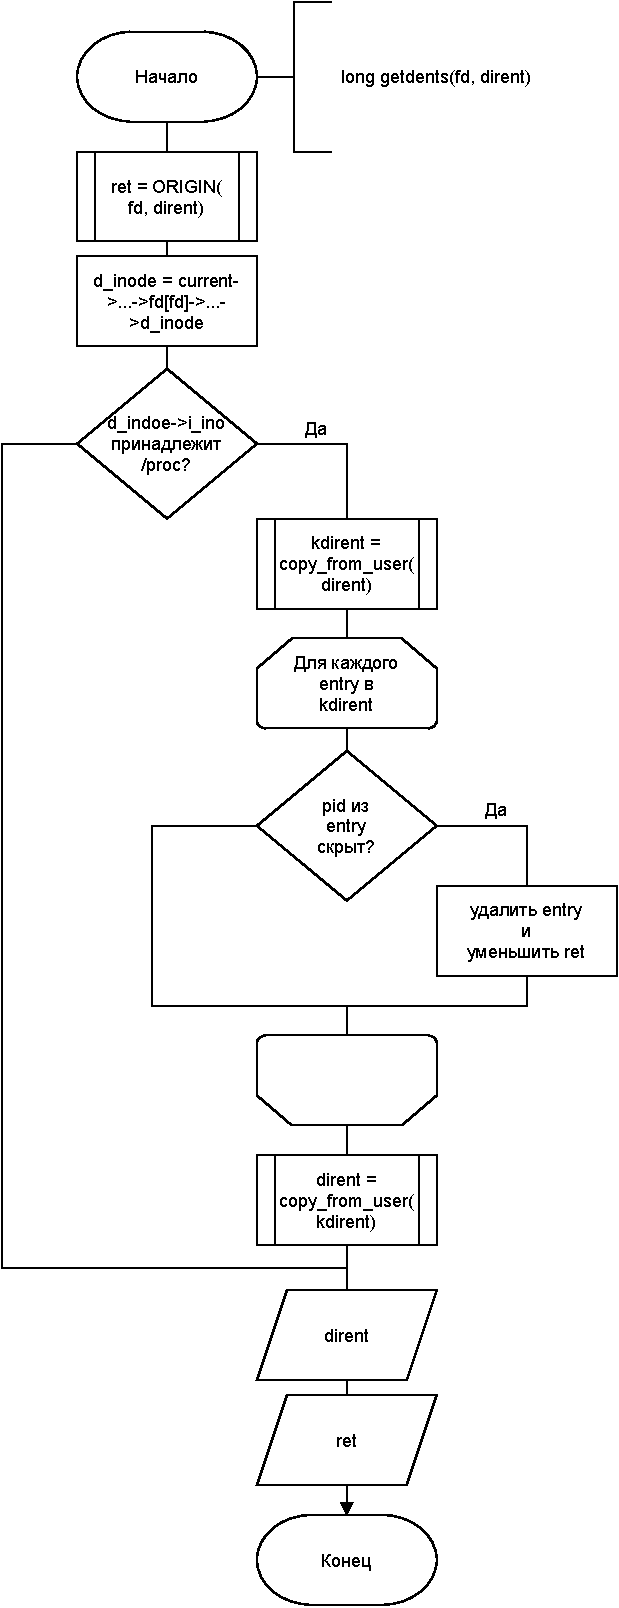
\includegraphics[scale=0.65]{pdf/oscw_proc.pdf}
    \caption{Схема алгоритма скрытия процесса}\label{img:proc_hide_scheme}
\end{figure}

\section{Скрытие сетевых сокетов}%
\label{sec:skrytie_setevykh_soketov}

Как показал анализ утилиты netstat при помощи программы strace, для отображения сетевых сокетов выполняется чтение /proc/net/tcp (tcp6, udp, udp6).

Для работы с файлами виртуальной файловой системы существуют специальный интерфейс~--- файловые последовательности, описываемые структурой struct seq\_file.

Для работы с файловыми последовательностями необходимо реализовать специальные функции. Для упомянутых выше файлов в ядре есть соответствующии им имплементации: tcp4\_seq\_show, udp4\_seq\_show, tcp6\_seq\_show, udp6\_seq\_show. В листинге~\ref{lst:tcp4_seq_show} представлен прототип одной из них.
\begin{lstlisting}[language=c,caption={Прототип tcp4\_seq\_show},label=lst:tcp4_seq_show]
int tcp4_seq_show(struct seq_file *seq, void *v);
\end{lstlisting}

Среди полей структуры struct seq\_file есть буфер buf, в который происходит запись содержимого файла. За каждый вызов упомянутой функции в этот буфер помещается новая строка.

В рассматриваемом случае, эта строка содержит информацию о сетевом подключении. Чтобы скрыть сетевой сокет, данную строку необходимо удалить из буфера, если в ней содержится номер порта, по которому происходит сокрытие сокета.

\begin{figure}[H]
    \centering
    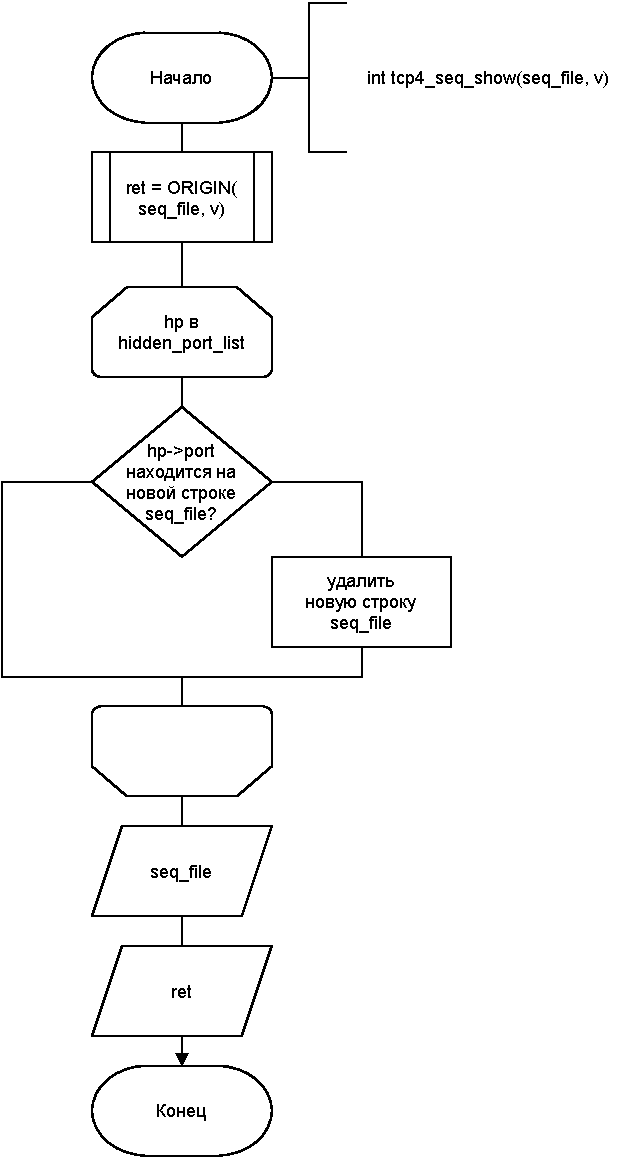
\includegraphics[scale=0.65]{pdf/oscw_net.pdf}
    \caption{Схема алгоритма скрытия сетевых сокетов}\label{img:net_hide_scheme}
\end{figure}

\section{Выводы}%
\label{sec:vyvody}

В данном разделе был рассмотрен процесс проектирования структуры программного обеспечения.
